\chapter{Adding Memory to the Agents}
\section{Overview}
Until now, we have assumed that all of the problems are fully observable, which means that they follow an MDP. The assumption behind this is that using the information given by the observation of the environment should be sufficient to fully understand its state. Thus:

\begin{equation}
    o_{t} = s_{t}
\end{equation}

But this is not always true and D-COACH is not suited to perform well in POMDPs. There are different reasons of why a problem is partially observed. In this work we focus on those cases where the observations represent instant information sensed from the environment but the state is described by time-dependent phenomena. For instance, if we want to estimate the velocity of a flying drone using information obtained from an RGB camera, it is necessary to combine data from different time steps in order to achieve this. 

In this chapter we aim to use a function approximation model that adds memory to the agents and to propose a variation of D-COACH which is capable of training this model. The idea is to validate this approach through simulations, establishing a baseline for further research in memory-based deep interactive learning.

\section{Method}
There are two well-known approaches for adding memory to agents in sequential decision-making problems when using DNNs as function approximator:

\begin{enumerate}
    \item \textbf{Observation stacking: \textbf{CITE}} This approach consists of stacking a fixed number of past observations to the current one and using this modified observation as the input of the policy. 
    \item \textbf{Recurrent models: \textbf{CITE}} This approach consists of using policies based on RNNs. Given that these models have an internal state, they can store information from the past (i.e. they have memory) and use it in posterior inferences. 
\end{enumerate}

One of the main issues of observation stacking is that the memory of this model is determined by the number of stacked observations. In high-dimensional state problems, the size of the input can increase considerably as the number of stacked observations increment, producing an overhead that makes this approach impractical. 

On the other hand, in RNNs the overhead is determined by the size of its hidden layers and the size of the sequences used when updating the weights of the model. As a consequence, the most important overhead of RNNs occurs when training. Several DRL approaches have used this approach without reporting large overheads \textbf{CITE}.

Given the more practical usage of recurrent models, in this work we use RNNs policies to test the viability of D-COACH for solving problems in a POMDP setting. 

\subsection{Learning to Remember}
Even though RNNs are networks with the capability of storing/summarizing information from past observations, they have to learn to do this. Commonly, in DRL approaches, this is not treated as a separated issue and the error of the cost function is propagated through the RNN as it would be done with other architectures. 

This may give the intuition that using D-COACH with RNNs would only require to change the FNN or CNN models with an RNN. Nevertheless, preliminary tests showed that shaping RNN-based policies with D-COACH made the agents to rapidly overfit to the first set of corrections, loosing the capability of learning interesting behaviors and, as a consequence, solving tasks. 

To overcome this shortcoming, we propose to use RNN layers to learn the dynamics of the environment, similarly as in \cite{Ha2018}. This approach take ideas from model-based RL in the sense that a model of the environment is learned. The difference is that in this case the model is learned such that the RNN layers learn to embed the past in its hidden state, but no planning or control techniques are used. In a nutshell, we want to learn the function $M(s_{t}, a_{t})$ as stated in Equation \ref{eq:model}:

\begin{equation}
    M(s_{t},a_{t}) = s_{t+1}
\end{equation}


\subsection{Low-dimensional State with Memory}
As it has been done previously in this work, we first study the low-dimensional state case. The objective is to learn the dynamics of the environment online i.e. as the policy is shaped interactively. 

If we look back to Chapter 2, the problem was similar. In that case the objective was to learn a low-dimensional embedding of a high-dimensional input online. The strategy was to share the encoder layers of an autoencoder between the policy and the autoencoder and update them using both the cost of the policy and the one of the autoencoder. In this case, we could see the hidden state of the recurrent layers as an embedding of past observations and share this layers between the policy and the model, updating them using both costs. The problem with this approach in this case is the one observed in the preliminary tests, the cost of the policy does not work well when updating the weights of recurrent layers.  

So, alternatively, the taken approach was to update the recurrent layers online only using the cost of the model and using the output of these layers as the input of FNN layers that are shaped using the policy cost. The model is updated with data collected while the agent is learning the policy. The general structure of this approach is shown in Figure \ref{fig:rnn_ld}.

\begin{figure}[h]
    \centering
    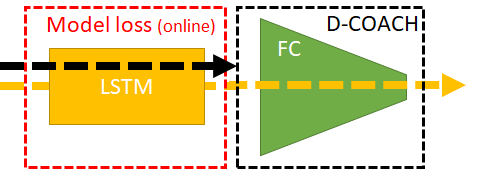
\includegraphics[width=0.5\linewidth]{imagenes/cap4/RNN_LD.png}
    \caption{Low-dimensional architecture for POMDP problems.}
    \label{fig:rnn_ld}
\end{figure}

The yellow arrow shows the flow of data when evaluating the network. The black arrow shows the flow of data when using the replay buffer to update the FNN layers. To train the FNN layers from the replay buffer a mini-batch is sampled, then is evaluated through the recurrent layers and finally is used as input of these layers (instead of directly storing the hidden state of the recurrent layers in the replay buffer).

\subsection{High-dimensional State with Memory}
In the high-dimensional case the agent needs to learn two embeddings: the one of the autoencoder, and the one of the model. In the preliminary tests, we found that the most effective way of doing this under the setting of D-COACH is to treat the autoencoder and the recurrent layers as one architecture, which represents the model. A model with the capability of learning from high-dimensional states, as it can be seen in Figure \ref{fig:rnn_hd}. 

\begin{figure}[h]
    \centering
    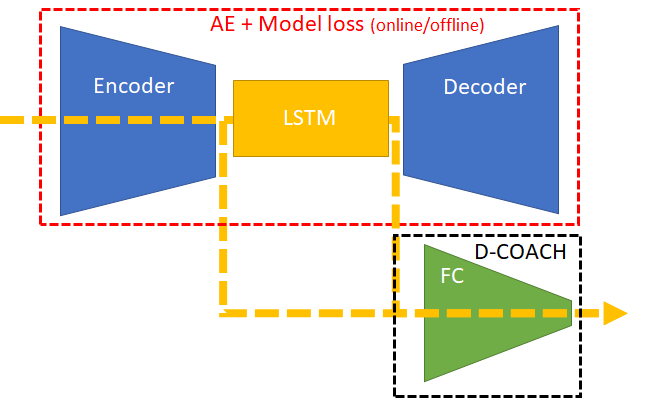
\includegraphics[width=0.6\linewidth]{imagenes/cap4/RNN_HD.png}
    \caption{High-dimensional architecture for POMDP problems.}
    \label{fig:rnn_hd}
\end{figure}

Instead of using a cost for the model and one for the autoencoder, we use the autoencoding cost but for reconstructing $s_{t+1}$. So, Equation \ref{eq:ae} instead of being $L(x_{t},\widetilde x_{t})$ it would be  $L(x_{t},\widetilde x_{t+1})$. The idea behind is to give memory to the autoencoder, so that can reconstruct future observations. By doing this, the output of the recurrent layers embed both the high-dimensional input and past observations.

\section{Experiments and Results}

\begin{figure}[h]
    \centering
    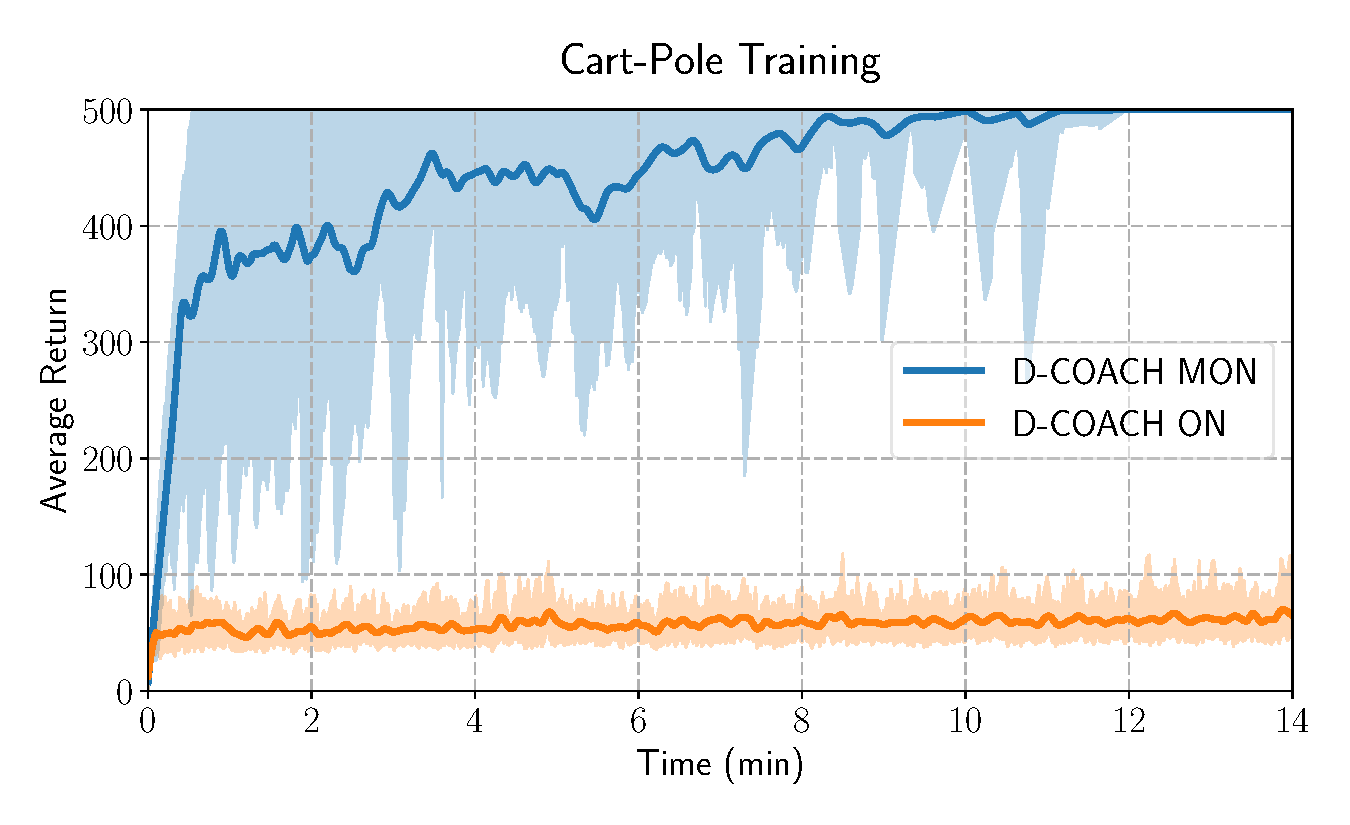
\includegraphics[width=0.9\linewidth]{imagenes/cap3/cartpole_LD_model.pdf}
    \caption{Evolution of the error while learning the reacher task. }
    \label{fig:reacher_exp}
\end{figure}

\begin{figure}[h]
    \centering
    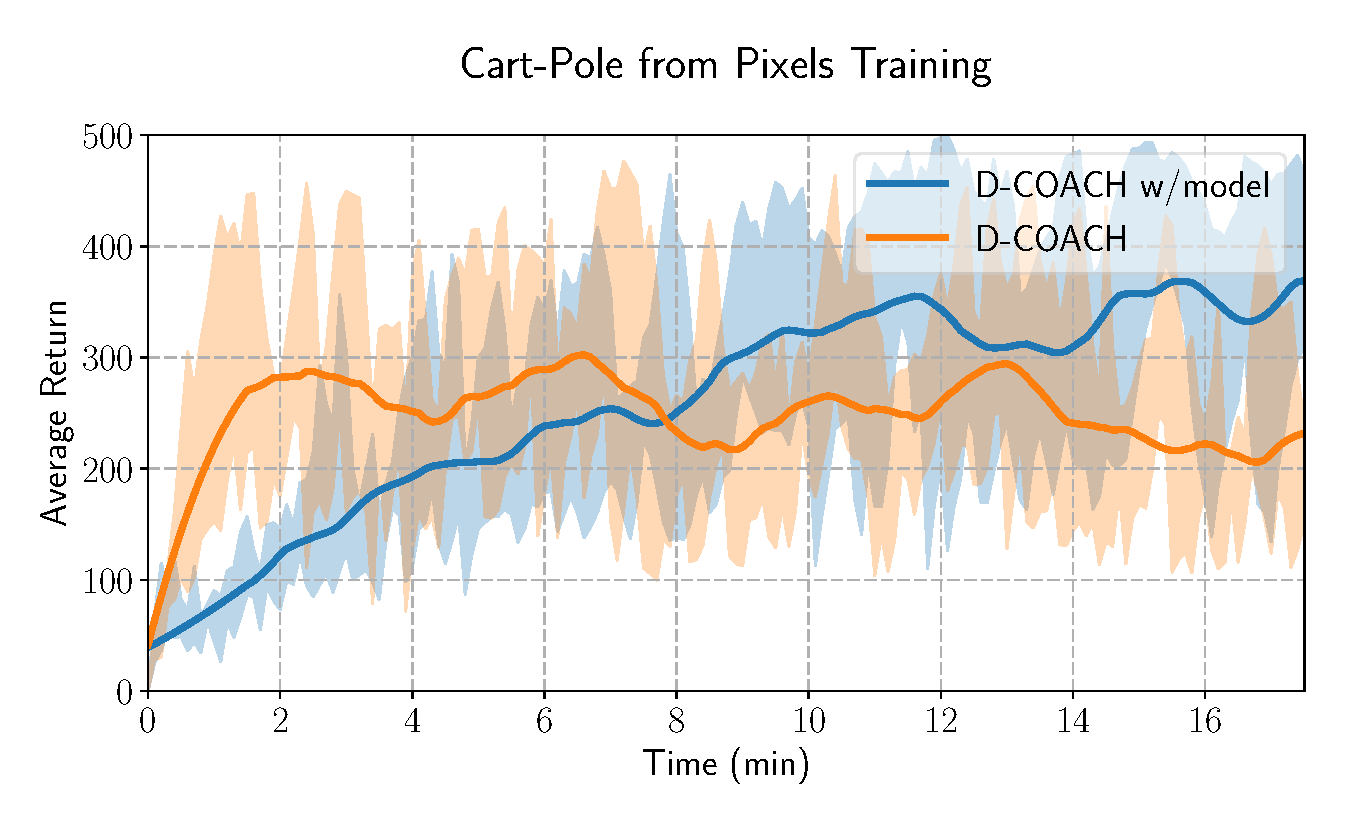
\includegraphics[width=0.9\linewidth]{imagenes/cap3/cartpole_HD_model.pdf}
    \caption{Evolution of the error while learning the reacher task. }
    \label{fig:reacher_exp}
\end{figure}


\begin{figure}[h]
    \centering
    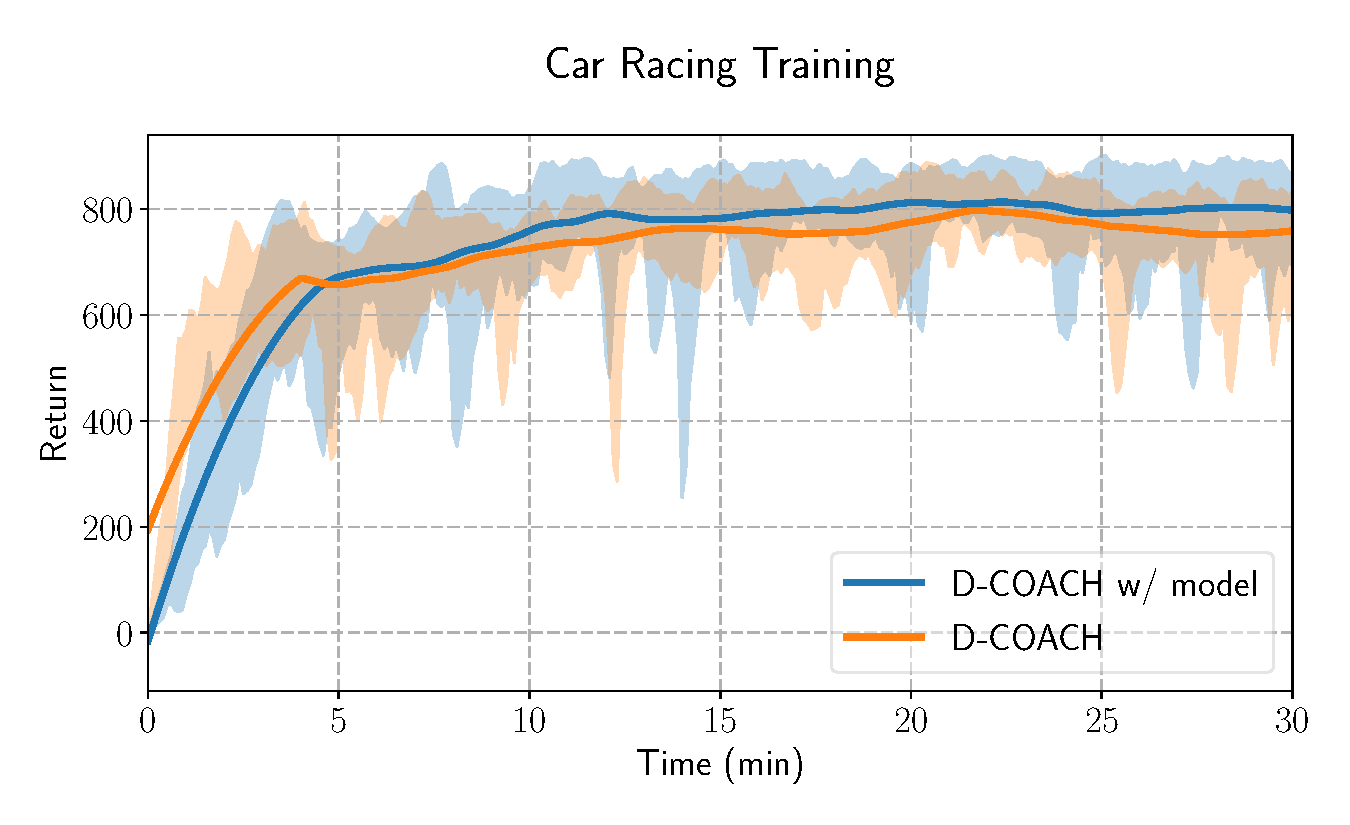
\includegraphics[width=0.9\linewidth]{imagenes/cap3/car_racing_lstm.pdf}
    \caption{Evolution of the error while learning the reacher task. }
    \label{fig:reacher_exp}
\end{figure}